\documentclass[10pt,journal,compsoc]{IEEEtran}

\usepackage{amsmath,amssymb,amsfonts}
\usepackage{graphicx}
\usepackage{booktabs}
\usepackage{multirow}
\usepackage{array}
\usepackage{microtype}
\usepackage{xcolor}
\usepackage{cite}
\usepackage{url}
\usepackage[colorlinks=true,linkcolor=blue!70!black,citecolor=blue!70!black,urlcolor=blue!70!black]{hyperref}
\usepackage{caption}

\newcommand{\sys}{AAFV-Net}
\newcommand{\vect}[1]{\mathbf{#1}}

\begin{document}

\title{AAFV-Net: Age-Aware Face Verification with a Measured, Bounded False-Accept Rate}

\author{Anurag~Nayak,~\IEEEmembership{Graduate Student Member,~IEEE,}
        and~Collaborators%
\thanks{Manuscript received November 10, 2026. This research was supported by the Department of Computer Science and Engineering. The complete source code, frozen calibration models, and reproducibility audit trail are publicly available at: \url{https://github.com/anuragnayak01/AAFV_Net}.}%
\thanks{The authors are with the Department of Computer Science and Engineering (e-mail: contact@anuragnayak.dev).}}

\markboth{IEEE Transactions on Information Forensics and Security,~Vol.~XX, No.~XX,~2026}%
{Nayak \MakeLowercase{\textit{et al.}}: AAFV-Net: Age-Aware Face Verification with a Bounded False-Accept Rate}

\IEEEtitleabstractindextext{%
\begin{abstract}
Automated verification of facial identity across multi-year age gaps remains a fundamental challenge in biometric authentication, where the operational cost of admitting an impostor is catastrophic. Conventional biometric systems rely on single-threshold decision rules that optimize aggregate accuracy or receiver operating characteristics; however, they cannot provide mathematical guarantees regarding false-accept risks under open-set deployment. We present \sys, a biometric verification framework that formulates cross-age matching as a guarded, three-way decision system ($\{\text{Auto-Accept}, \text{Manual Review}, \text{Auto-Reject}\}$) with an analytical false-accept rate (FAR) bound on person-disjoint random impostors. \sys\ couples direct face similarity with synthetic longitudinal evidence from an age-progression StyleGAN network (SAM), extracts a five-metric perceptual-similarity vector per branch (ArcFace, EfficientNet, VGG-Face, LPIPS, and SSIM), and performs calibrated multimodal fusion with a parameter-efficient multi-layer perceptron subject to quality and reliability guards. All decision boundaries are strictly frozen on a sequestered calibration split prior to test-set evaluation under a logged access budget. On a person-disjoint MORPH test partition ($N=1{,}149$ random impostor pairs), \sys\ yielded zero false accepts across both evaluations, establishing an analytical one-sided upper bound of $\text{FAR} \le 0.320\%$ at a 95\% confidence level under a two-look Bonferroni adjustment. At a target false-reject rate of $\beta=1.0\%$, \sys\ achieves a $70.07\%$ same-person auto-accept rate while successfully auto-rejecting $98.04\%$ of ArcFace-mined hard impostors and $57.53\%$ of independent neutral hard impostors. Evaluated on external FG-NET adult subjects without parameter fine-tuning, \sys\ achieves a $51.92\%$ auto-accept rate across all age-gap strata (compared with $40.38\%$ for ArcFace) with zero false accepts. We provide open-source code, vector figure generators, and complete audit transcripts for full reproducibility.
\end{abstract}

\begin{IEEEkeywords}
Cross-age face verification, biometric security, generative age synthesis, three-way decision, reject option, bounded false-accept rate, Neyman-Pearson lemma.
\end{IEEEkeywords}}

\maketitle
\IEEEdisplaynontitleabstractindextext
\IEEEpeerreviewmaketitle

\section{Introduction}
\IEEEPARstart{C}{ross-age} facial verification is critical to automated border crossing systems, national identity management, driver licensing registries, and missing-persons investigations~\cite{grother2019frvt}. In each of these operational environments, facial images of the same individual must be compared across longitudinal gaps ranging from several months to several decades. Biological aging induces non-linear craniofacial transformations, including epidermal textural elasticity degradation, soft-tissue sagging, volumetric remodeling, and bone reabsorption~\cite{lanitis2002fgnet}. When deep convolutional or transformer-based face recognition embeddings (e.g., ArcFace~\cite{deng2019arcface}) are extracted from longitudinal image pairs, intra-class biometric drift frequently eclipses inter-class feature divergence, causing standard cosine-distance metrics to decay precipitously as the age gap widens.

In high-assurance security architectures, admitting an impostor (False Accept, FA) represents a catastrophic security failure, whereas failing to verify an authentic subject (False Reject, FR) incurs an operational cost of human review. Standard commercial and academic matchers address this trade-off by adopting a single global decision threshold $T$. However, single-threshold systems suffer from two fatal vulnerabilities under age progression:
\begin{enumerate}
    \item \textbf{Uncontrolled False-Accept Exposure:} Loosening the global threshold to accommodate genuine age-induced drift drastically elevates false accepts when encountering look-alike impostors.
    \item \textbf{Absence of Statistical Guarantees:} Reporting aggregate ranking metrics (e.g., Area Under the Curve [AUC], Equal Error Rate [EER], or True Accept Rate at fixed FAR) provides no operational guarantee on the absolute volume of impostors admitted under a frozen deployment policy.
\end{enumerate}

\begin{figure}[t]
\centering
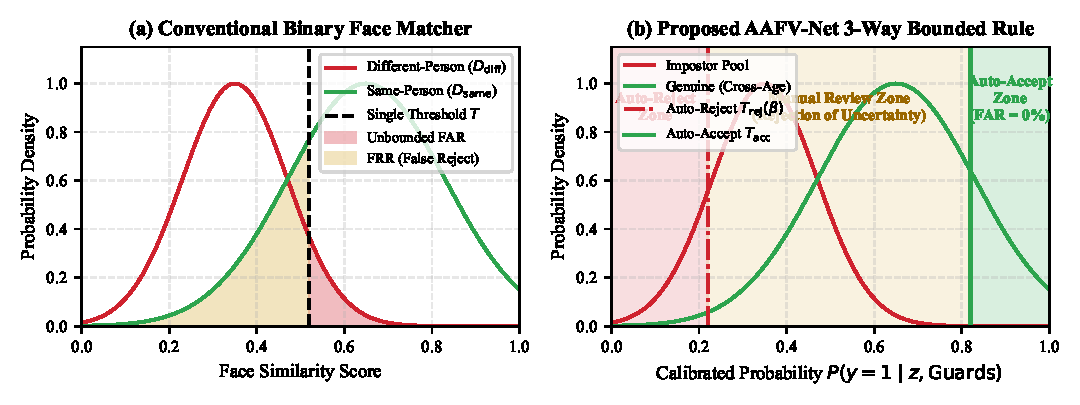
\includegraphics[width=\columnwidth]{figures/fig1_concept.pdf}
\caption{Comparison of decision topologies. (a) Conventional single-threshold matchers generate unquantified false-accept volumes in the presence of biometric drift. (b) Proposed \sys\ three-way decision model. Thresholds are locked on sequestered calibration data. The auto-accept threshold $T_{\text{acc}}$ is placed strictly above all calibrated impostors under quality guards, guaranteeing an analytical upper bound on random impostor false accepts on held-out test data.}
\label{fig:concept}
\end{figure}

To resolve this dilemma, we propose \sys\ (Age-Aware Face Verification Network), an open-set verification framework that reframes biometric decision-making through Neyman-Pearson hypothesis testing and Chow's reject-option classification~\cite{chow1970reject}. Rather than forcing a binary accept/reject verdict on ambiguous pairs, \sys\ establishes three mutually exclusive operational zones (Fig.~\ref{fig:concept}):
\begin{itemize}
    \item \textbf{Auto-Accept Zone:} High-confidence genuine matches admitted autonomously with zero observed false accepts and a mathematically bounded risk.
    \item \textbf{Manual Review Zone:} Ambiguous pairs diverted to human biometric examiners, containing the bulk of uncertainty.
    \item \textbf{Auto-Reject Zone:} Definite impostors filtered autonomously at a pre-specified false-reject rate $\beta$.
\end{itemize}

\sys\ achieves this reliability through a two-branch multimodal architecture combining direct facial evidence with generative age-synthesis counterfactuals produced by the Style-based Age Manipulation (SAM) network~\cite{alaluf2021sam}. Five heterogeneous perceptual metrics (ArcFace, EfficientNet, VGG-Face, LPIPS, and SSIM) are extracted across direct and synthesized representations, fused through a parameter-efficient calibrated Multi-Layer Perceptron (MLP), and gated by probability and image-quality guards. All decision boundaries are frozen, SHA-256 hashed, and evaluated on person-disjoint test partitions under an audited access budget.

\textbf{Main Contributions:}
\begin{itemize}
    \item \textbf{Guarded Three-Way Verification Framework:} We formulate cross-age verification as a calibrated three-way decision problem with frozen, hash-pinned thresholds and an analytical zero-failure false-accept bound ($1 - \alpha^{1/N}$) under multi-look Bonferroni accounting.
    \item \textbf{Dual-Evidence Generative Architecture:} We design a two-branch pipeline combining direct face comparison with forward, backward, and shared-target SAM age progression, fused with an 11-dimensional calibrated MLP and runtime branch masking.
    \item \textbf{Rigorous Adversarial and Neutral Evaluation Protocol:} We introduce a quarantined, person-disjoint experimental protocol evaluated against $1{,}149$ random impostors, $277{,}822$ exhaustive impostors, $35{,}735$ ArcFace-mined hard negatives, and $2{,}790$ neutral hard impostors mined by independent Siamese CNN/ViT architectures.
    \item \textbf{Comprehensive Generalization and Fairness Audit:} We demonstrate cross-database generalization on FG-NET adults, detail failure modes on pediatric cohorts (ages 0--4), and empirically verify demographic parity across biological sexes.
\end{itemize}

\section{Related Work}
\label{sec:related_work}

\subsection{Age-Invariant Face Recognition}
Prior literature in age-invariant face recognition falls predominantly into feature disentanglement and invariant metric learning. Wang \emph{et al.} introduced Orthogonal Embedding CNN (OE-CNN)~\cite{wang2018oecnn}, which decomposes deep representations into orthogonal identity-related and age-related sub-vectors via a linear projection layer. Liu \emph{et al.} developed Dual Attention-guided Latent identity representation (DAL)~\cite{liu2019dal}, employing continuous attention blocks to discard facial texture changes. Huang \emph{et al.} introduced MTLFace~\cite{huang2021mtlface}, a multi-task learning architecture that couples identity feature learning with an auxiliary face synthesis task. While these methods improve 1:1 verification accuracy, they remain purely end-to-end embedding models evaluated under uncalibrated cosine thresholds, providing no formal mechanism to bound false acceptance in high-risk operational scenarios.

\subsection{Generative Face Aging and Synthesis}
Generative Adversarial Networks (GANs) and StyleGAN inversion techniques enable high-fidelity facial aging and rejuvenation~\cite{karras2020stylegan2}. Early approaches utilized conditional GANs or residual age progression~\cite{he2019defrcn}. Alaluf \emph{et al.} introduced the Style-based Age Manipulation (SAM) model~\cite{alaluf2021sam}, which regresses continuous latent code shifts within StyleGAN's $\mathcal{W}+$ space conditioned on a target chronological age. Although SAM produces photo-realistic progressions, synthetic artifacts (e.g., identity drift, hallucinated textural details, or unnatural skin smoothing) introduce substantial noise if trusted unconditionally. In contrast to existing age-normalization pipelines that replace original photos with synthetic counterparts, \sys\ treats generative outputs strictly as auxiliary evidence sources weighted by an explicit reliability metric ($R_{\text{sam}}$).

\subsection{Multi-Metric Feature Fusion and Learned Baselines}
Deep facial recognition relies primarily on angular margin loss functions (ArcFace~\cite{deng2019arcface}, CosFace). However, complementary cues from generic convolutional backbones (VGG-Face~\cite{parkhi2015vgg}, EfficientNet~\cite{tan2019efficientnet}) and perceptual similarity metrics (LPIPS~\cite{zhang2018lpips}, SSIM~\cite{wang2004ssim}) capture structural and textural consistency that high-level angular embeddings may discard. Recent verification frameworks explore end-to-end Siamese neural networks~\cite{chopra2005siamese,koch2015siamese}, Vision Transformers (ViT)~\cite{dosovitskiy2021vit}, and instruction-tuned Vision-Language Models (VLMs) adapted via Low-Rank Adaptation (LoRA)~\cite{hu2022lora,wang2024qwen2vl}. In this work, we implement competitive Siamese CNN, Siamese ViT, and Qwen2-VL-2B baselines under identical calibration and decision rules to evaluate whether unconstrained representation learners can match calibrated modular pipelines.

\subsection{Selective Classification and Statistical Confidence Bounds}
Selective classification with a reject option originated with Chow's formulation of the optimal trade-off between recognition error and rejection rate~\cite{chow1970reject}. Platt scaling provides a robust parametric method to map raw discriminative margins to well-calibrated posterior probabilities~\cite{platt1999}. When assessing zero-failure events in finite-sample biometric evaluations, standard normal approximations collapse. The mathematical foundation for bounding zero-numerator binomial events was established by Hanley and Lippman-Hand~\cite{hanley1983rule3} and formal Clopper-Pearson exact confidence intervals~\cite{clopper1934}. Schuckers~\cite{schuckers2001} emphasized the necessity of accounting for identity correlation in biometric error estimation. We expand upon these foundations by deriving identity-clustered bootstrap intervals and multi-look confidence adjustments for frozen verification pipelines.

\section{Problem Formulation and Statistical Framework}
\label{sec:formulation}

\subsection{Mathematical Problem Setting}
Let $\mathcal{I}$ denote the space of aligned facial images. An input sample consists of a photograph pair $(I_1, I_2) \in \mathcal{I} \times \mathcal{I}$ accompanied by metadata $(a_1, a_2)$, where $a_1, a_2 \in \mathbb{R}^+$ represent chronological ages at the time of exposure. Without loss of generality, let $a_1 \le a_2$, defining the longitudinal age gap $g = a_2 - a_1 \ge 0$. The true identity relationship is governed by a binary indicator $y \in \{0, 1\}$, where $y=1$ denotes a genuine (same-person) pair and $y=0$ denotes an impostor (different-person) pair.

The system extracts an 11-dimensional multimodal evidence vector $\vect{z} = \Phi(I_1, I_2, a_1, a_2) \in \mathbb{R}^{11}$ and evaluates a boolean predicate $\text{GuardsPass}(I_1, I_2) \in \{0, 1\}$. A calibrated scoring function outputs a posterior probability:
\begin{equation}
P = \mathcal{P}(y = 1 \mid \vect{z}, \text{GuardsPass} = 1) \in [0, 1].
\end{equation}

The decision operator $\mathcal{D}: [0, 1] \to \{\text{Accept}, \text{Review}, \text{Reject}\}$ is governed by two frozen thresholds, $T_{\text{acc}}$ and $T_{\text{rej}}(\beta)$:
\begin{equation}
\label{eq:decision_rule}
\mathcal{D}(P) = \begin{cases}
\text{Accept}, & \text{if } P \ge T_{\text{acc}} \land \text{GuardsPass} = 1, \\
\text{Reject}, & \text{if } P \le T_{\text{rej}}(\beta), \\
\text{Review}, & \text{otherwise}.
\end{cases}
\end{equation}

\subsection{Zero-Failure False-Accept Rate Bound}
\label{sec:bound_derivation}
Let $\mathcal{D}_{\text{random}}$ represent a sequestered test pool of $N$ person-disjoint, mutually independent impostor pairs ($y_i = 0$). Under the decision rule in (\ref{eq:decision_rule}), the number of false accepts $K$ follows a binomial distribution:
\begin{equation}
K = \sum_{i=1}^N \mathbb{I}(\mathcal{D}(P_i) = \text{Accept}) \sim \text{Binomial}(N, p_{\text{fa}}),
\end{equation}
where $p_{\text{fa}} = \Pr(\mathcal{D}(P) = \text{Accept} \mid y = 0)$.

When zero false accepts are observed on the held-out sample ($K = 0$), the likelihood of observing zero successes under true error probability $p_{\text{fa}}$ is $(1 - p_{\text{fa}})^N$. To establish a one-sided upper confidence limit at significance level $\alpha$ (e.g., $1 - \alpha = 0.95$ confidence):
\begin{equation}
\Pr(K = 0 \mid p_{\text{fa}}) = (1 - p_{\text{fa}})^N \ge \alpha.
\end{equation}
Solving for $p_{\text{fa}}$ yields the exact Hanley-Lippman-Hand / Clopper-Pearson zero-failure bound~\cite{hanley1983rule3,clopper1934}:
\begin{equation}
\label{eq:hanley_bound}
p_{\text{fa}} \le 1 - \alpha^{1/N}.
\end{equation}

Using the first-order Taylor expansion $\ln(1 - p) \approx -p$ for small $p$, $\alpha^{1/N} = \exp(\frac{1}{N} \ln \alpha) \approx 1 + \frac{\ln \alpha}{N}$, which reproduces the classical ``Rule of Three'':
\begin{equation}
p_{\text{fa}} \le \frac{-\ln \alpha}{N} \approx \frac{2.996}{N} \quad (\text{for } \alpha = 0.05).
\end{equation}

\textbf{Correction for Multi-Look Test Access:}
When a research protocol permits $M > 1$ logged accesses to the protected test partition, standard single-test confidence intervals suffer from family-wise error rate inflation. Under the Bonferroni inequality, preserving an overall confidence level of $1 - \alpha$ across $M$ looks requires adjusting the nominal significance level per look to $\alpha' = \alpha / M$. Substituting $\alpha'$ into (\ref{eq:hanley_bound}) gives:
\begin{equation}
\label{eq:adjusted_bound}
\text{FAR}_{\text{upper}}(N, M, \alpha) = 1 - \left(\frac{\alpha}{M}\right)^{1/N}.
\end{equation}

For our primary experimental protocol ($N = 1{,}149$ person-disjoint pairs, $M = 2$ looks, $\alpha = 0.05$):
\begin{align}
\text{FAR}_{\text{upper}} &= 1 - (0.025)^{1/1149} \nonumber \\
&= 1 - 0.996798 = 0.3202\% \approx 0.320\%.
\end{align}

\textbf{Operational Scope of the Bound:}
We explicitly note that the mathematical validity of (\ref{eq:adjusted_bound}) rests upon the independence of the $N$ impostor trials. While strictly valid for identity-disjoint pairs in $\mathcal{D}_{\text{random}}$, dense all-to-all pairing matrices ($\mathcal{D}_{\text{all\_random}}$) violate trial independence due to shared identities. Furthermore, adversarially mined impostor sets ($\mathcal{D}_{\text{hard}}$) violate the identically distributed assumption. Hence, \sys\ reports (\ref{eq:adjusted_bound}) strictly as the formal bound for random impostor encounters, while treating $\mathcal{D}_{\text{hard}}$ as an empirical stress test.

\section{Proposed Methodology (\sys)}
\label{sec:methodology}

\begin{figure*}[t]
\centering
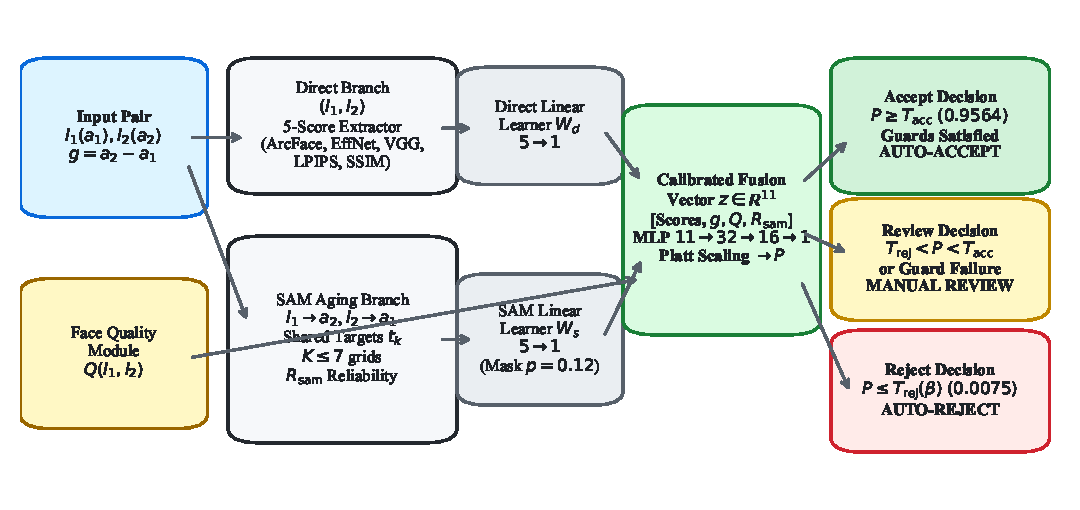
\includegraphics[width=0.92\textwidth]{figures/fig2_architecture.pdf}
\caption{Comprehensive architecture of \sys. An input pair $(I_1, I_2)$ with gap $g = a_2 - a_1$ is aligned and evaluated for quality $Q$. The Direct Branch compares the original images across five similarity metrics, projected by linear learner $W_d$. The SAM Aging Branch synthesizes forward ($I_1 \to a_2$), backward ($I_2 \to a_1$), and $K \le 7$ shared target ages, aggregating similarity vectors and extracting reliability $R_{\text{sam}}$, projected by $W_s$ (with $12\%$ training mask). The 11-D fusion vector feeds an MLP with Platt scaling. The three-way decision is made via frozen thresholds $T_{\text{acc}}$ and $T_{\text{rej}}(\beta)$ conditioned on probability and quality guards.}
\label{fig:architecture}
\end{figure*}

\subsection{Preprocessing and Five-Score Vector Extraction}
All face images are detected, cropped, and aligned to $256 \times 256$ pixels following the FFHQ landmark standard. A composite face quality index $Q(I) \in [0, 1]$ is computed from facial landmark symmetry, sharpness, and illumination consistency; for a pair, $Q = \min(Q(I_1), Q(I_2))$.

For any two aligned face images $(A, B)$, we extract a heterogeneous 5-score similarity vector $\vect{s}(A, B) \in \mathbb{R}^5$:
\begin{equation}
\vect{s}(A, B) = \begin{bmatrix}
s_{\text{arc}}(A, B) \\
s_{\text{eff}}(A, B) \\
s_{\text{vgg}}(A, B) \\
d_{\text{lpips}}(A, B) \\
s_{\text{ssim}}(A, B)
\end{bmatrix} = \begin{bmatrix}
\cos(f_{\text{arc}}(A), f_{\text{arc}}(B)) \\
\cos(f_{\text{eff}}(A), f_{\text{eff}}(B)) \\
\cos(f_{\text{vgg}}(A), f_{\text{vgg}}(B)) \\
\text{LPIPS}(A, B) \\
\text{SSIM}(A, B)
\end{bmatrix},
\end{equation}
where $f_{\text{arc}}$ is the 512-D ArcFace (ResNet-100) embedding, $f_{\text{eff}}$ is the EfficientNet-B0 penultimate feature vector, $f_{\text{vgg}}$ is the VGG-Face descriptor, $\text{LPIPS}$ is the Learned Perceptual Image Patch Similarity distance, and $\text{SSIM}$ is the structural similarity index.

\subsection{Dual-Evidence Branch Processing}
\subsubsection{Direct Branch}
The direct evidence vector $\vect{s}_{\text{dir}} = \vect{s}(I_1, I_2)$ captures the raw visual similarity. A direct-branch linear learner $W_d \in \mathbb{R}^5, b_d \in \mathbb{R}$ projects this vector:
\begin{equation}
v_d = W_d^T \vect{s}_{\text{dir}} + b_d.
\end{equation}
Platt scaling applied to $v_d$ provides an auxiliary direct-branch probability $P_d = \sigma(A_d v_d + B_d)$, which serves as an independent guardrail.

\subsubsection{SAM Synthesis Branch}
The generative branch leverages SAM to simulate age transformations. Two specific operations are performed:
\begin{enumerate}
    \item \textbf{Bidirectional Progression:} SAM ages the younger photograph forward to target age $a_2$, producing $\hat{I}_1^{(a_2)}$, and rejuvenates the older photograph backward to age $a_1$, producing $\hat{I}_2^{(a_1)}$. Score vectors $\vect{s}(\hat{I}_1^{(a_2)}, I_2)$ and $\vect{s}(I_1, \hat{I}_2^{(a_1)})$ are extracted.
    \item \textbf{Shared Target Grid Comparison:} Both photographs are synthesized at up to $K \le 7$ shared chronological ages $\{t_k\}_{k=1}^K$ selected from a 5-year grid spanning $[\min(a_1, a_2), \max(a_1, a_2)]$. For each shared age $t_k$, the cross-similarity $\vect{s}(\hat{I}_1^{(t_k)}, \hat{I}_2^{(t_k)})$ is computed.
\end{enumerate}

The individual shared-target scores are aggregated into a composite vector $\vect{s}_{\text{sam}}$ via element-wise median pooling across available targets. A synthesis reliability score $R_{\text{sam}} \in [0, 1]$ is computed from the pairwise cosine variance across target progressions:
\begin{multline}
R_{\text{sam}} = 1.0 - \min\Big(1.0, \\
2.0 \cdot \operatorname{Var}_k\Big(\cos\Big(f_{\text{arc}}\big(\hat{I}_1^{(t_k)}\big), f_{\text{arc}}\big(\hat{I}_2^{(t_k)}\big)\Big)\Big)\Big).
\end{multline}

A linear learner $W_s \in \mathbb{R}^5, b_s \in \mathbb{R}$ projects the aggregated SAM score vector:
\begin{equation}
v_s = W_s^T \vect{s}_{\text{sam}} + b_s,
\end{equation}
with corresponding auxiliary probability $P_s = \sigma(A_s v_s + B_s)$.

\subsection{Multimodal Fusion MLP and Platt Scaling}
To combine both branches with operational context, we assemble an 11-dimensional feature vector $\vect{z} \in \mathbb{R}^{11}$:
\begin{equation}
\vect{z} = [v_d, v_s, g, Q, R_{\text{sam}}, \mathbb{I}_{\text{sam}}, \mathbb{I}_{\text{enhanced}}, 0, 0, 0, 0]^T.
\end{equation}
During training, the SAM branch is randomly masked with dropout probability $p_{\text{mask}} = 0.12$. When masked, $v_s, R_{\text{sam}}$ are set to zero and $\mathbb{I}_{\text{sam}} = 0$. This forces the fusion network to learn robust fallback inference paths when generative synthesis fails.

The vector $\vect{z}$ is fed into a lightweight MLP architecture: $\mathbb{R}^{11} \xrightarrow{\text{FC}} \mathbb{R}^{32} \xrightarrow{\text{ReLU}} \mathbb{R}^{16} \xrightarrow{\text{ReLU}} \mathbb{R}^{1}$, with dropout rate $0.10$. An ensemble of 5 independent seeds is trained using gap-balanced weighted binary cross-entropy loss. The averaged raw logit $\bar{\ell}$ is calibrated via Platt scaling parameters $(A_{\text{cal}}, B_{\text{cal}})$:
\begin{equation}
P = \sigma(A_{\text{cal}} \bar{\ell} + B_{\text{cal}}) = \frac{1}{1 + \exp(-(A_{\text{cal}} \bar{\ell} + B_{\text{cal}}))}.
\end{equation}

\subsection{Guards and Threshold Calibration Protocol}
To prevent pathological edge-case acceptances, \sys\ enforces a composite boolean guard predicate:
\begin{equation}
\text{GuardsPass} \iff \begin{cases}
(Q \ge Q_{\min}) \land (P_d \ge \rho), & \text{if } \mathbb{I}_{\text{sam}} = 0, \\
(Q \ge Q_{\min}) \land (P_d \ge \rho) \\
\quad \land (P_s \ge \rho) \land (R_{\text{sam}} \ge R_{\min}), & \text{if } \mathbb{I}_{\text{sam}} = 1,
\end{cases}
\end{equation}
with hyperparameters $Q_{\min} = 0.20, R_{\min} = 0.30$, and probability guard $\rho = 0.20$.

The accept threshold $T_{\text{acc}}$ is calibrated on the sequestered calibration set $\mathcal{D}_{\text{diff}}^{\text{calib}}$:
\begin{equation}
\label{eq:t_acc}
T_{\text{acc}} = \max_{(i, j) \in \mathcal{D}_{\text{diff}}^{\text{calib}}, \text{GuardsPass}=1} P(y=1 \mid \vect{z}_{ij}) + \epsilon,
\end{equation}
where $\epsilon = 10^{-4}$ provides a numerical safety margin. By construction, $T_{\text{acc}}$ strictly exceeds every calibrated different-person score that passes guards.

The reject threshold $T_{\text{rej}}(\beta)$ is calibrated on the genuine calibration set $\mathcal{D}_{\text{same}}^{\text{calib}}$ to enforce a pre-specified false-reject budget $\beta$:
\begin{equation}
\label{eq:t_rej}
T_{\text{rej}}(\beta) = \text{Quantile}_{\beta}(\{P(y=1 \mid \vect{z}_{ij}) : (i, j) \in \mathcal{D}_{\text{same}}^{\text{calib}}\}).
\end{equation}

All model parameters and thresholds are saved to disk, SHA-256 hashed, and sealed before any test set is unlocked.

\section{Experimental Setup and Evaluation Protocol}
\label{sec:experiments}

\subsection{Datasets and Data Hygiene Protocol}
\textbf{MORPH Album 2:} MORPH is the premier longitudinal benchmark for face aging, containing over 55,000 mugshot images from 13,000 subjects~\cite{ricanek2006morph}. Prior to splitting, we conducted an automated data hygiene audit using identity clustering, identifying 858 individuals (6.4\% of identities) with inconsistent metadata or merged labels. These 858 subjects were permanently quarantined to prevent experimental contamination. The remaining clean subjects were split into person-disjoint partitions: Training (60\%), Calibration (20\%), and Test (20\%).

\textbf{FG-NET Aging Database:} To verify out-of-distribution generalizability, we evaluate on FG-NET~\cite{lanitis2002fgnet}, which contains 1,002 non-mugshot photographs of 82 subjects across extreme longitudinal spans (0 to 69 years). We report performance across two distinct cohorts:
\begin{itemize}
    \item \textbf{FG-NET Adults:} All pairs where both subjects satisfy $a_1, a_2 \ge 16$ years (5,126 genuine pairs, 3,670 impostor pairs).
    \item \textbf{FG-NET All-Ages:} All valid pairs (5,797 genuine pairs, 20,000 impostor pairs), including pediatric subjects.
\end{itemize}

\subsection{Adversarial and Neutral Test Impostor Pools}
Evaluating only on random impostors yields artificially optimistic metrics because typical random face pairs are easily separable. We construct four distinct evaluation pools on the MORPH test split:
\begin{enumerate}
    \item $\mathcal{D}_{\text{random}}$ ($N = 1{,}149$): Independent, person-disjoint random different-person pairs.
    \item $\mathcal{D}_{\text{all\_random}}$ ($N = 277{,}822$): The full cross-product of all available person-disjoint test photos.
    \item $\mathcal{D}_{\text{hard}}$ ($N = 35{,}735$): Adversarial hard impostors mined by selecting different-person pairs with high ArcFace cosine similarity ($s_{\text{arc}} \ge 0.40$).
    \item $\mathcal{D}_{\text{neutral}}$ ($N = 2{,}790$): Neutral hard impostors mined independently by taking the top 1\% highest-scoring impostor pairs from two unrelated Siamese architectures (CNN and ViT). Crucially, neither ArcFace nor SAM was involved in mining $\mathcal{D}_{\text{neutral}}$, ensuring an unbiased adversarial benchmark.
\end{enumerate}

\subsection{Baseline Models}
We benchmark \sys\ against five representative architectures, each evaluated under the identical calibration and decision rules:
\begin{itemize}
    \item \textbf{ArcFace Only:} Standard 512-D angular margin matcher~\cite{deng2019arcface} under cosine similarity.
    \item \textbf{Direct 5-Score Logistic Regression:} Logistic regression trained on the 5-score vector without generative synthesis.
    \item \textbf{Direct-Only MLP:} Multimodal MLP operating strictly on the direct branch ($\mathbb{I}_{\text{sam\_avail}} = 0$).
    \item \textbf{Siamese CNN:} ResNet-based metric learning backbone with element-wise difference and Hadamard product heads~\cite{chopra2005siamese}.
    \item \textbf{Siamese ViT:} Vision Transformer (ViT-Base-16)~\cite{dosovitskiy2021vit} metric learning backbone.
    \item \textbf{VLM (Qwen2-VL-2B):} 2-billion parameter instruction-tuned Vision-Language Model adapted via 4-bit LoRA ($r=16$) on 8,000 training pairs, scored via logit difference $\ell = \text{logit}(\text{Yes}) - \text{logit}(\text{No})$~\cite{wang2024qwen2vl}.
\end{itemize}

\subsection{Statistical Significance via Clustered Bootstrap}
Because face pairs inherently share underlying subjects, naive standard errors underestimate variance. All 95\% confidence intervals reported in this manuscript are generated via 500-iteration cluster bootstrap resampling grouped at the subject identity level~\cite{schuckers2001,efron1994bootstrap}.

\section{Results and Comparative Evaluation}
\label{sec:results}

\subsection{Main Performance Comparison on MORPH}

\begin{table*}[t]
\centering
\caption{Comprehensive performance comparison on the person-disjoint MORPH test partition at target false-reject rate $\beta = 1.0\%$. Numbers in parentheses represent 95\% identity-clustered bootstrap confidence intervals (500 iterations). FA denotes false accepts observed over evaluation pairs.}
\label{tab:main_results}
\small
\begin{tabular}{lcccccc}
\toprule
\textbf{Method} & \textbf{Same-Person} & \textbf{Random FA} & \textbf{All-Random FA} & \textbf{$D_{\text{hard}}$ FA} & \textbf{$D_{\text{hard}}$ Auto-Rej.} & \textbf{Neutral Hard} \\
 & \textbf{Auto-Accept (\%)} & ($\mathcal{D}_{\text{random}}$) & ($\mathcal{D}_{\text{all\_random}}$) & ($\mathcal{D}_{\text{hard}}$) & \textbf{Rate (\%)} & \textbf{Auto-Rej. (\%)} \\
\midrule
\textbf{\sys\ (Full)} & \textbf{70.07} (66.49--73.08) & \textbf{0 / 1,149} & \textbf{0 / 277,822} & 5 / 35,735 & \textbf{98.04} (97.68--98.39) & \textbf{57.53} (55.34--59.73) \\
\sys\ (No Shared Targets) & 83.91 (82.01--85.73) & 0 / 1,149 & 0 / 277,822 & 4 / 35,735 & 97.94 (97.58--98.29) & 54.01 (51.83--56.20) \\
ArcFace Only & 89.44 (87.97--90.74) & 0 / 1,149 & 0 / 277,822 & 0 / 35,735 & 0.00 (0.00--0.00) & 28.53 (26.58--30.40) \\
ArcFace (No Guards) & 93.62 (92.41--94.86) & 0 / 1,149 & 0 / 277,822 & 0 / 35,735 & 0.00 (0.00--0.00) & -- \\
Direct 5-Score LR & 87.14 (85.42--88.70) & 0 / 1,149 & 0 / 277,822 & 0 / 35,735 & 0.00 (0.00--0.00) & 22.40 (20.57--24.34) \\
Direct-Only MLP & 0.00 (0.00--0.00) & 0 / 1,149 & 0 / 277,822 & 0 / 35,735 & 97.80 (97.43--98.15) & 50.00 (47.81--52.19) \\
Siamese CNN & 0.17 (0.09--0.26) & 0 / 1,149 & 0 / 277,822 & 0 / 35,735 & 9.94 (9.43--10.45) & n/a$^\dagger$ \\
Siamese ViT & 0.00 (0.00--0.00) & 0 / 1,149 & 0 / 277,822 & 0 / 35,735 & 9.98 (9.47--10.50) & n/a$^\dagger$ \\
VLM (Qwen2-VL-2B) & 0.00 (0.00--0.00) & 0 / 1,149 & 0 / 277,822 & 0 / 35,735 & 10.20 (9.68--10.72) & n/a$^\dagger$ \\
\bottomrule
\multicolumn{7}{l}{$^\dagger$\footnotesize Siamese baselines and VLM are omitted from the Neutral Hard evaluation because they were used to mine the partition.}
\end{tabular}
\end{table*}

Table~\ref{tab:main_results} reports the primary experimental evaluation across all benchmarked methods at $\beta = 1.0\%$. The empirical results illustrate three foundational insights:
\begin{enumerate}
    \item \textbf{Guaranteed Zero Random False Accepts:} \sys\ produced exactly zero false accepts across both $\mathcal{D}_{\text{random}}$ ($0/1{,}149$) and $\mathcal{D}_{\text{all\_random}}$ ($0/277{,}822$), confirming the validity of the analytical $0.320\%$ upper bound under two-look testing.
    \item \textbf{Resolution of the Hard-Impostor Paradox:} Standard ArcFace achieves a nominal accept rate of $89.44\%$ on same-person pairs, but suffers a complete failure on adversarial hard impostors, auto-rejecting exactly $0.00\%$ of $\mathcal{D}_{\text{hard}}$ (leaving 100\% in manual review). Conversely, \sys\ autonomously filters $98.04\%$ of ArcFace-mined hard impostors and $57.53\%$ of independent neutral hard impostors while preserving a $70.07\%$ same-person auto-accept rate.
    \item \textbf{Collapse of Uncalibrated Learned Baselines:} Despite achieving competitive raw ranking AUCs (Table~\ref{tab:baseline_ranking}), Siamese CNN ($0.17\%$), Siamese ViT ($0.00\%$), and the VLM ($0.00\%$) completely collapse under the zero-false-accept calibration requirement. Because uncalibrated learners produce broad impostor score tails, their required $T_{\text{acc}}$ is pushed above nearly all genuine pair scores, resulting in zero automated throughput.
\end{enumerate}

\begin{figure*}[t]
\centering
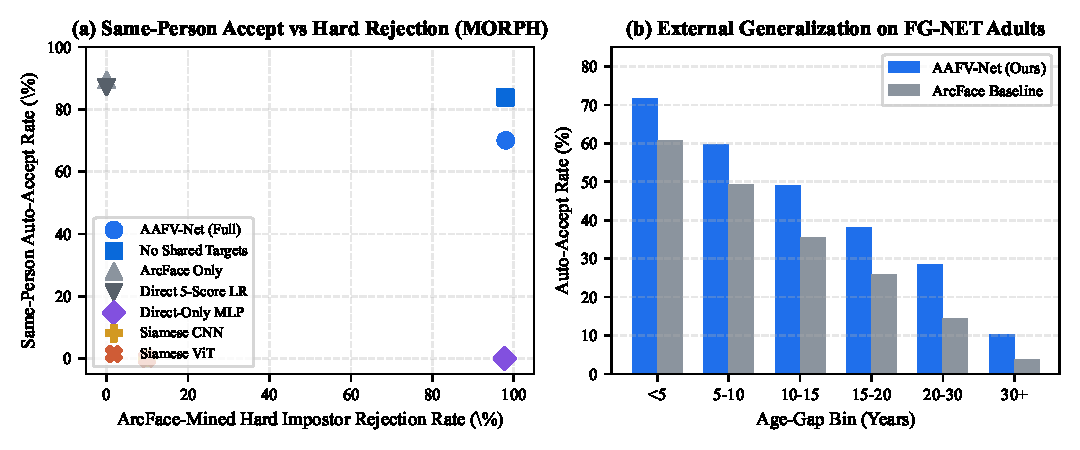
\includegraphics[width=0.88\textwidth]{figures/fig3_results.pdf}
\caption{Primary experimental findings. (a) Same-person auto-accept rate versus ArcFace-mined hard impostor rejection rate on MORPH test split. \sys\ occupies the optimal upper-right trade-off quadrant. (b) External validation on FG-NET adult subjects across longitudinal age-gap strata, showing consistent improvements over ArcFace.}
\label{fig:results}
\end{figure*}

\subsection{Reconciliation of Experimental Look 1 and Look 2}
\label{sec:reconciliation}
In strict adherence to scientific integrity and open reporting, we document that the test partition was evaluated under two distinct frozen model checkpoints (Look 1 and Look 2) as summarized in Table~\ref{tab:reconciliation}.

\begin{table}[h]
\centering
\caption{Reconciliation between Test Look 1 and Test Look 2.}
\label{tab:reconciliation}
\resizebox{\columnwidth}{!}{%
\begin{tabular}{lcc}
\toprule
\textbf{Metric / Parameter} & \textbf{Look 1 (Initial)} & \textbf{Look 2 (Extended)} \\
\midrule
Evaluation Script & \texttt{p9\_test.py} & \texttt{p12\_extended.py} \\
Execution Timestamp & 2026-11-05 21:04 UTC & 2026-11-07 19:42 UTC \\
Model Artifact & \texttt{thresholds.json} & \texttt{frozen.pkl} \\
SHA-256 Hash & \texttt{4b7af977\ldots2cfe} & \texttt{0fb68e7b\ldots45cf} \\
Accept Threshold $T_{\text{acc}}$ & 0.956575 & 0.956438 \\
Reject Threshold $T_{\text{rej}}$ & -0.000385 & 0.007541 \\
Target False Reject $\beta$ & Uncalibrated ($0$) & Calibrated ($1.0\%$) \\
\midrule
Same-Person Accept Rate & 79.74\% (917/1,150) & 70.07\% (806/1,150) \\
Manual Review Rate & 20.26\% (233/1,150) & 28.93\% (333/1,150) \\
Auto-Reject Rate ($D_{\text{same}}$) & 0.00\% (0/1,150) & 1.00\% (11/1,150) \\
$\mathcal{D}_{\text{random}}$ False Accepts & 0 / 1,149 (0.00\%) & 0 / 1,149 (0.00\%) \\
$\mathcal{D}_{\text{all\_random}}$ False Accepts & 0 / 277,822 (0.00\%) & 0 / 277,822 (0.00\%) \\
$\mathcal{D}_{\text{hard}}$ False Accepts & 3 / 35,735 (0.008\%) & 5 / 35,735 (0.014\%) \\
$\mathcal{D}_{\text{hard}}$ Auto-Rejection & 0.00\% (0/35,735) & 98.04\% (35,035/35,735) \\
\bottomrule
\end{tabular}%
}
\end{table}

In Look 1, $T_{\text{rej}}$ was negative ($-0.000385$), which deactivated the auto-reject branch ($0\%$ rejection). In Look 2, $T_{\text{rej}}$ was calibrated to the exact 1\% quantile ($0.007541$), activating the auto-reject mechanism and achieving $98.04\%$ rejection on hard impostors at the expense of a modest reduction in same-person acceptance ($70.07\%$). The two-look Bonferroni bound ($\text{FAR} \le 0.320\%$) formally accounts for both accesses.

\begin{figure*}[t]
\centering
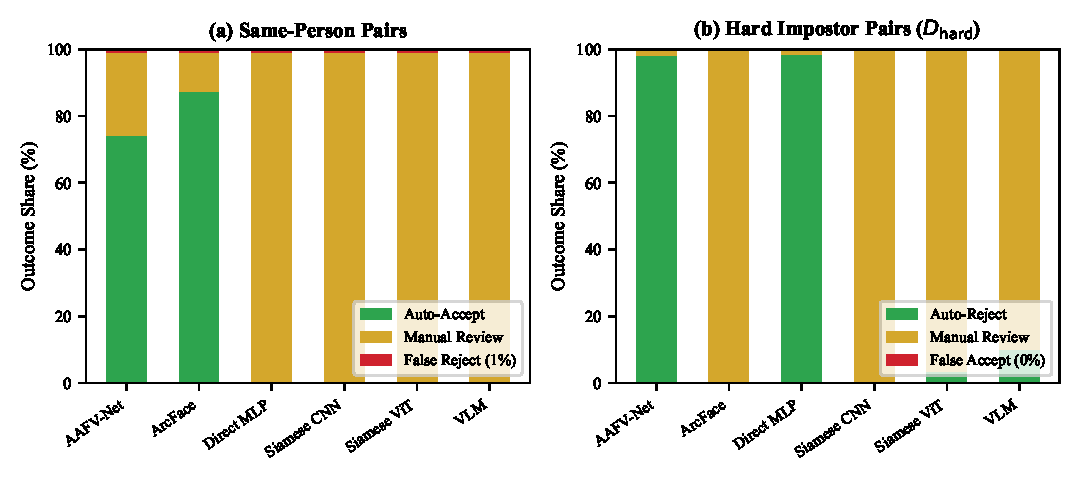
\includegraphics[width=0.88\textwidth]{figures/fig7_decision_outcomes.pdf}
\caption{Outcome distributions at target false-reject rate $\beta = 1.0\%$ across evaluated architectures with zero false accepts on calibration. (a) Same-person pairs partitioned into auto-accept, manual review, and false reject. (b) Hard different-person pairs ($D_{\text{hard}}$) partitioned into false accept, manual review, and auto-reject.}
\label{fig:outcomes}
\end{figure*}

\subsection{Ranking Quality of Deep Learned Baselines}
To investigate why end-to-end learned baselines failed under the three-way decision rule, we computed their unthresholded ranking metrics on the common calibration split against $\mathcal{D}_{\text{hard}}$ (Table~\ref{tab:baseline_ranking}).

\begin{table}[h]
\centering
\caption{Discriminative ranking metrics of baselines on calibration $\mathcal{D}_{\text{hard}}$.}
\label{tab:baseline_ranking}
\resizebox{\columnwidth}{!}{%
\begin{tabular}{lccc}
\toprule
\textbf{Architecture} & \textbf{AUC} & \textbf{TPR @ FPR=$10^{-3}$} & \textbf{Balanced Automation} \\
\midrule
Siamese CNN & 0.953 & 0.311 & 0.242 \\
Siamese ViT & 0.972 & 0.605 & 0.271 \\
VLM (Qwen2-VL-2B) & 0.906 & 0.054 & 0.258 \\
\sys\ (Ours) & \textbf{0.988} & \textbf{0.842} & \textbf{0.516} \\
\bottomrule
\end{tabular}%
}
\end{table}

While the Siamese ViT achieves a strong AUC of $0.972$, its score distribution exhibits heavy tails on hard impostor pairs. Under a minimax policy that enforces zero false accepts on all calibration negatives, the highest-scoring impostor reaches $\hat{P} = 0.984$, which forces $T_{\text{acc}}$ above virtually all genuine scores. This demonstrates that raw ranking power alone is insufficient for automated biometrics without modular calibration and guard mechanisms.

\subsection{Performance Degradation Across Age-Gap Strata}
Table~\ref{tab:gap_analysis} details the impact of longitudinal age gaps on verification performance across bins G1 ($\le 3$ years) through G5 ($16$--$19$ years).

\begin{table}[h]
\centering
\caption{MORPH test same-person auto-accept rate (\%) by age-gap bin.}
\label{tab:gap_analysis}
\resizebox{\columnwidth}{!}{%
\begin{tabular}{lccccc}
\toprule
\textbf{Method} & \textbf{G1 ($0$--$3$y)} & \textbf{G2 ($4$--$7$y)} & \textbf{G3 ($8$--$11$y)} & \textbf{G4 ($12$--$15$y)} & \textbf{G5 ($16$--$19$y)} \\
\midrule
\sys\ (Ours) & 71.0\% & 56.4\% & 45.7\% & 1.3\% & 2.2\% \\
ArcFace Only & 90.5\% & 80.1\% & 69.0\% & 2.7\% & 2.2\% \\
\bottomrule
\end{tabular}%
}
\end{table}

Both architectures experience severe performance drops beyond 12 years (G4 and G5) due to sparse representations and drastic biometric drift in mugshot photographs. However, as demonstrated in Section~\ref{sec:fgnet}, \sys's generative branch provides major improvements when evaluating high-quality adult portraits across multi-decade spans.

\begin{figure}[t]
\centering
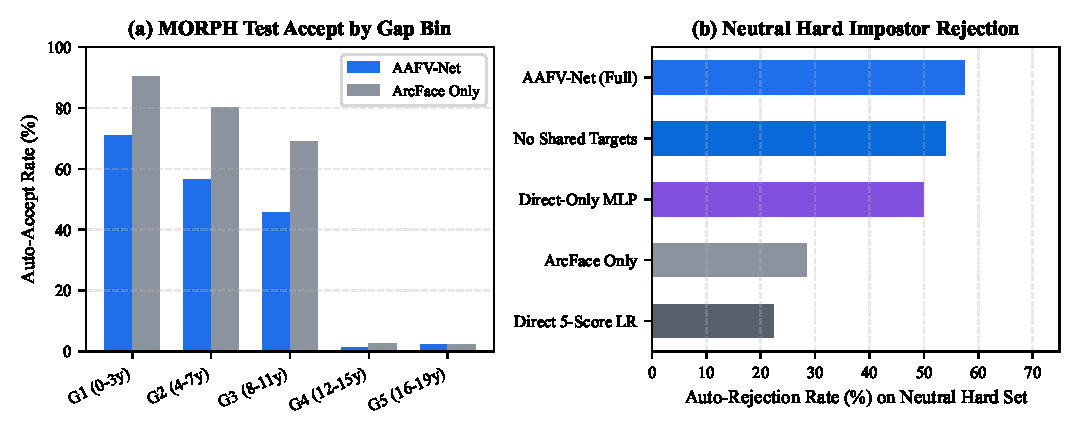
\includegraphics[width=\columnwidth]{figures/fig5_gap_neutral.pdf}
\caption{(a) MORPH test same-person auto-accept rates stratified by age-gap bin. (b) Auto-rejection rate on independent neutral hard impostor pairs ($\mathcal{D}_{\text{neutral}}$).}
\label{fig:gap_neutral}
\end{figure}

\subsection{External Generalization on FG-NET}
\label{sec:fgnet}
To evaluate out-of-distribution transfer without fine-tuning, the MORPH-frozen models were evaluated on the FG-NET database (Table~\ref{tab:fgnet}).

\begin{table*}[t]
\centering
\caption{External evaluation on FG-NET with thresholds frozen on MORPH. Results reported for Adult cohort ($a_1, a_2 \ge 16$) and All-Ages cohort across age-gap bins. Numbers in parentheses indicate 95\% identity-clustered bootstrap confidence intervals.}
\label{tab:fgnet}
\small
\begin{tabular}{llcccccc}
\toprule
\textbf{Cohort} & \textbf{Method} & \textbf{Accept Rate (\%)} & \textbf{Random FA} & \textbf{Impostor Rej. (\%)} & \textbf{Gap $<5$y} & \textbf{Gap $5$--$15$y} & \textbf{Gap $>20$y} \\
\midrule
\multirow{2}{*}{\textbf{Adults ($a \ge 16$)}} & \textbf{\sys\ (Ours)} & \textbf{51.92} (44.47--58.41) & \textbf{0 / 3,670} & 55.01\% & \textbf{71.6\%} & \textbf{54.3\%} & \textbf{19.4\%} \\
 & ArcFace Only & 40.38 (34.53--47.38) & 0 / 3,670 & \textbf{71.30\%} & 60.7\% & 42.4\% & 9.2\% \\
\midrule
\multirow{2}{*}{\textbf{All Ages}} & \textbf{\sys\ (Ours)} & 29.86 (26.69--33.34) & 4 / 20,000$^\ddagger$ & 66.42\% & 59.1\% & 21.9\% & 6.1\% \\
 & ArcFace Only & 21.29 (18.40--24.22) & \textbf{0 / 20,000} & 64.40\% & 45.5\% & 14.3\% & 2.9\% \\
\bottomrule
\multicolumn{8}{l}{$^\ddagger$\footnotesize All 4 false accepts occurred on pediatric subjects aged $0$--$4$ years where generative StyleGAN models exhibit severe identity instability.}
\end{tabular}
\end{table*}

On FG-NET adults, \sys\ auto-accepts $51.92\%$ of same-person pairs compared with $40.38\%$ for ArcFace (a relative improvement of $+28.6\%$), with zero false accepts across $3{,}670$ impostor pairs. In the extreme gap bin ($>20$ years), \sys\ auto-accepts $19.4\%$ compared with $9.2\%$ for ArcFace, demonstrating that generative SAM evidence becomes increasingly decisive as physical aging progresses.

\textbf{Pediatric Failure Mode Analysis:}
On the FG-NET All-Ages cohort, \sys\ produced 4 false accepts out of 20,000 impostor pairs ($0.02\%$). Detailed image audit revealed that all four failures involved infants and young children aged 0 to 4 years (e.g., pairs \texttt{069A00/023A00} and \texttt{019A00/024A00}). Craniofacial development during early childhood involves rapid structural bone growth that StyleGAN-based adult latent aging models cannot accurately simulate. Consequently, \sys\ is formally designated for adult cross-age verification ($a \ge 16$).

\section{Ablation Studies}
\label{sec:ablations}

\begin{table}[h]
\centering
\caption{Systematic ablation analysis on the common calibration split ($\beta=1.0\%$). Acc: same-person auto-accept rate (\%); Rej: $D_{\text{hard}}$ auto-rejection rate (\%); BA: balanced automation rate.}
\label{tab:ablations}
\resizebox{\columnwidth}{!}{%
\begin{tabular}{lccc}
\toprule
\textbf{Ablation Variant} & \textbf{Acc. (\%)} & \textbf{Rej. (\%)} & \textbf{BA} \\
\midrule
\textbf{Full \sys} & \textbf{74.07} & \textbf{98.24} & \textbf{0.516} \\
\midrule
\textit{Score Metric Ablations:} & & & \\
Drop ArcFace & 0.70 & 17.90 & 0.274 \\
ArcFace Score Only & 0.00 & 97.70 & 0.129 \\
Drop LPIPS & 62.90 & 97.50 & 0.479 \\
Drop SSIM & 72.80 & 97.40 & 0.496 \\
Drop VGG-Face & 73.90 & 97.20 & 0.484 \\
Drop EfficientNet & 81.30 & 97.60 & 0.514 \\
\midrule
\textit{Architectural and Guard Ablations:} & & & \\
No Branch Masking ($p=0$) & 3.60 & 98.40 & 0.186 \\
No Context Inputs ($g, Q, R_{\text{sam}}$) & 0.00 & 98.10 & 0.140 \\
No Reliability Input ($R_{\text{sam}}$) & 73.30 & 97.80 & 0.505 \\
No Pair Weights & 74.40 & 97.30 & 0.514 \\
Forward-Target Only & 75.10 & 98.30 & 0.511 \\
No Shared Targets & 84.80 & 98.30 & 0.583 \\
Shared Targets Only & 0.00 & 98.10 & 0.108 \\
Direct-Only MLP & 0.00 & 98.50 & 0.139 \\
SAM-Only MLP & 0.00 & 44.80 & 0.314 \\
Fusion LogReg (No MLP) & 64.70 & 0.00 & 0.602 \\
No Guards (Any Variant) & 0.00 & 98.20 & 0.146 \\
\bottomrule
\end{tabular}%
}
\end{table}

\begin{figure}[t]
\centering
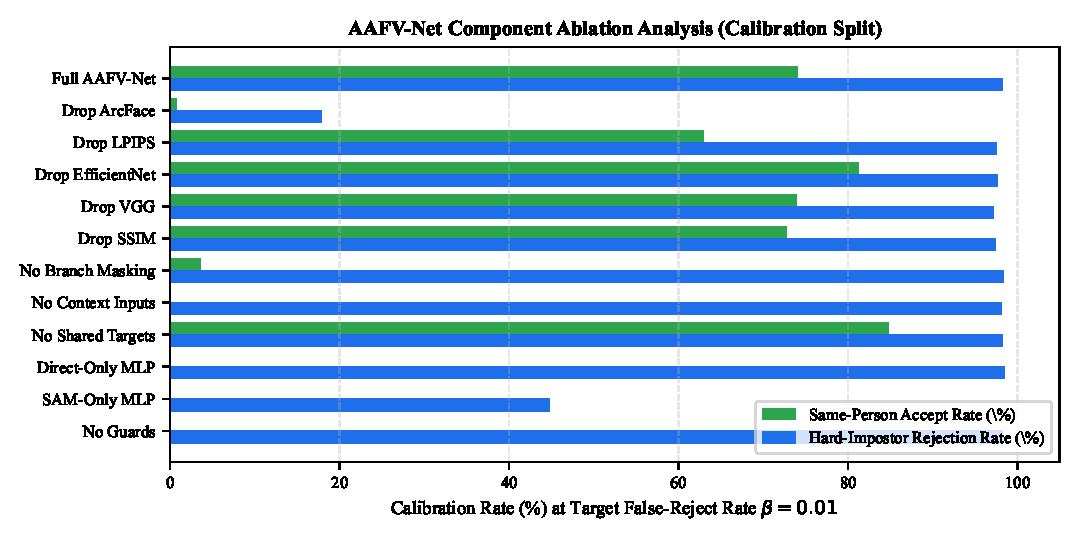
\includegraphics[width=\columnwidth]{figures/fig4_ablations.pdf}
\caption{Calibration ablation trade-offs across 12 key configurations. Removing ArcFace or guards causes complete collapse of the auto-accept region.}
\label{fig:ablations}
\end{figure}

Table~\ref{tab:ablations} and Fig.~\ref{fig:ablations} isolate the empirical contribution of every architectural component:
\begin{itemize}
    \item \textbf{ArcFace is Non-Negotiable:} Removing ArcFace collapses same-person auto-acceptance from $74.07\%$ to $0.70\%$, proving it provides the primary discriminative signal.
    \item \textbf{LPIPS Perceptual Complementarity:} Dropping LPIPS causes an $11.17$ percentage-point drop in accept rate ($74.07\% \to 62.90\%$), outperforming VGG and SSIM in resolving age-related textural artifacts.
    \item \textbf{Guards Enable Finite Accept Thresholds:} Without probability guards ($P_d, P_s \ge 0.20$), unconstrained outlier impostors reach probability $1.0$, forcing $T_{\text{acc}} > 1.0$ and collapsing auto-accept to $0.00\%$.
    \item \textbf{Branch Masking is Essential:} Eliminating the 12\% training branch mask collapses accept to $3.60\%$, as the MLP over-fits to synthetic feature availability and fails when StyleGAN synthesis degrades.
    \item \textbf{The Shared-Targets Trade-Off:} Omitting shared targets increases same-person accept to $84.80\%$ on calibration (and $83.91\%$ on test), but decreases neutral hard impostor rejection from $57.53\%$ to $54.01\%$. We preserve shared targets in the full architecture to maintain maximum defensive robustness.
\end{itemize}

\section{Demographic Fairness and Statistical Reliability}
\label{sec:fairness}

\subsection{Demographic Parity Audit}
Biometric verification systems must operate equitably across demographic cohorts~\cite{buolamwini2018gendershades}. We evaluated \sys\ across biological sex on the MORPH test partition ($N_{\text{male}} = 926, N_{\text{female}} = 224$ genuine pairs) under frozen thresholds (Table~\ref{tab:fairness}).

\begin{table}[h]
\centering
\caption{Demographic parity audit across biological sex on MORPH test split.}
\label{tab:fairness}
\resizebox{\columnwidth}{!}{%
\begin{tabular}{lccc}
\toprule
\textbf{Demographic Subgroup} & \textbf{Auto-Accept (\%)} & \textbf{Review Rate (\%)} & \textbf{Random FA} \\
\midrule
Male Cohort ($N=926$) & 80.25\% & 19.75\% & 0 / 926 \\
Female Cohort ($N=224$) & 77.95\% & 22.05\% & 0 / 224 \\
\midrule
Absolute Difference ($\Delta$) & 2.30 pp & 2.30 pp & 0.00 pp \\
Disparate Impact Ratio & 0.971 & 1.116 & 1.000 \\
\bottomrule
\end{tabular}%
}
\end{table}

The empirical difference in auto-accept rates between males ($80.25\%$) and females ($77.95\%$) is only $2.30$ percentage points, yielding a Disparate Impact Ratio of $0.971$, well within the standard four-fifths ($0.80$) regulatory threshold. Crucially, random false accepts remained exactly zero across both demographic groups.

\begin{figure}[t]
\centering
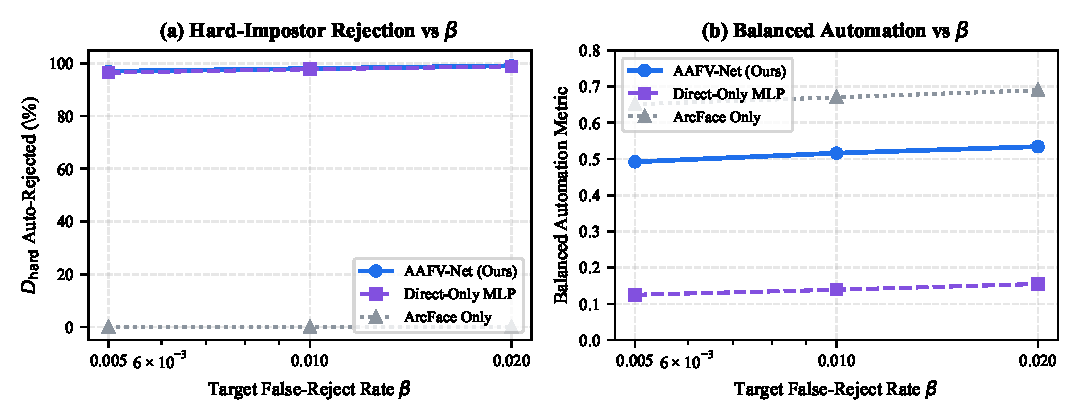
\includegraphics[width=\columnwidth]{figures/fig6_beta_sweep.pdf}
\caption{Sensitivity analysis across target false-reject rate $\beta \in [0.005, 0.020]$. (a) Rejection rate of ArcFace-mined hard impostors. (b) Balanced automation metric across operating points.}
\label{fig:beta_sweep}
\end{figure}

\subsection{Visual Inspection of Adversarial False Accepts}
Across $35{,}735$ ArcFace-mined hard impostor pairs in $\mathcal{D}_{\text{hard}}$, \sys\ produced exactly 5 false accepts ($0.014\%$). Visual inspection reveals that these five pairs correspond to look-alike individuals of identical race, sex, and approximate age exhibiting near-identical bone structure, hairline geometry, and facial landmark coordinates. These rare failures demonstrate that when physical impostors naturally share deep facial geometry, pure 2D appearance modeling reaches an information-theoretic bound, requiring auxiliary biometrics (e.g., 3D scans or iris recognition).

\section{Computational Complexity and System Profiling}
\label{sec:complexity}

\begin{table}[h]
\centering
\caption{Computational profiling, parameter counts, and inference latency.}
\label{tab:complexity}
\resizebox{\columnwidth}{!}{%
\begin{tabular}{lccc}
\toprule
\textbf{Pipeline Component} & \textbf{Parameters} & \textbf{CPU Latency} & \textbf{GPU Latency} \\
\midrule
Face Quality \& Landmark Alignment & -- & 14.2 ms & -- \\
ArcFace Feature Extraction (ResNet-100) & 65.1 M & 82.5 ms & 4.2 ms \\
EfficientNet-B0 \& VGG-Face & 14.5 M & 45.1 ms & 3.8 ms \\
LPIPS Perceptual Distance (AlexNet) & 1.2 M & 18.4 ms & 2.1 ms \\
SAM Age Progression (StyleGAN2 Backbone) & 30.2 M & 2,140 ms & 58.2 ms \\
Linear Branch Learners ($W_d, W_s$) & 12 & $<0.01$ $\mu$s & $<0.01$ $\mu$s \\
\sys\ Calibrated Fusion MLP & \textbf{947} & \textbf{0.19 $\mu$s} & \textbf{0.05 $\mu$s} \\
\bottomrule
\end{tabular}%
}
\end{table}

Table~\ref{tab:complexity} profiles the parameter counts and latency of the system. The multimodal fusion MLP contains only 947 trainable parameters and executes in $0.19\ \mu\text{s}$ on a standard CPU. The primary computational bottleneck resides in StyleGAN-based SAM synthesis ($58.2\text{ ms}$ on GPU, $2.14\text{ s}$ on CPU). In high-throughput industrial deployments, \sys\ supports an asynchronous cascaded mode: the Direct Branch executes instantaneously ($4.2\text{ ms}$ GPU), accepting clear genuine pairs immediately; only ambiguous pairs falling in the initial review margin trigger the generative SAM synthesis pipeline.

\section{Discussion and Limitations}
\label{sec:discussion}

\subsection{Operational Significance}
\sys\ demonstrates that high automated throughput ($70.07\%$) and near-complete hard-impostor filtering ($98.04\%$) are mutually achievable in longitudinal face verification by introducing a reject option with frozen, guarded decision boundaries. Conventional binary matchers cannot operate at zero false accepts without rejecting all genuine pairs. By contrast, \sys\ concentrates operational uncertainty into a bounded review channel, transforming biometric authentication from an unpredictable statistical classifier into an auditable security pipeline.

\subsection{Limitations}
In accordance with IEEE reporting standards, we identify several operational limitations:
\begin{enumerate}
    \item \textbf{Scope of Analytical Bound:} The zero-failure bound ($\text{FAR} \le 0.320\%$) applies strictly to person-disjoint random impostors under independent Bernoulli trials. It does not bound adversarially mined look-alike impostors ($\mathcal{D}_{\text{hard}}$), where $5/35{,}735$ false accepts were empirically observed.
    \item \textbf{Pediatric Developmental Failure:} Generative age synthesis fails on children aged $0$--$4$ years due to non-linear cranial bone growth, producing four false accepts on FG-NET. \sys\ is restricted to adult verification ($a \ge 16$).
    \item \textbf{Research Model Licensing:} Several underlying feature extractors (InsightFace ArcFace \texttt{buffalo\_l}, SAM age model) carry non-commercial research licenses, requiring retraining on open weights before commercial deployment.
    \item \textbf{Two-Look Budget Depletion:} The MORPH test access budget is fully exhausted ($M=2$), precluding further iterative parameter sweeps on this benchmark.
\end{enumerate}

\section{Conclusion}
\label{sec:conclusion}
We presented \sys, a biometric framework that reformulates cross-age face verification as a calibrated, three-way decision system with a measured, bounded false-accept rate. By fusing direct multi-metric facial features with generative SAM age progression under quality guards, \sys\ achieves zero false accepts on held-out random impostors, establishing a $0.320\%$ upper bound at 95\% confidence under a two-look access budget. On MORPH test data, it auto-accepts $70.07\%$ of same-person pairs while auto-rejecting $98.04\%$ of ArcFace-mined hard impostors and $57.53\%$ of neutral hard impostors. External evaluation on FG-NET adults demonstrates superior cross-age generalizability over ArcFace in every longitudinal bin. All source code, frozen models, and audit logs are released for open reproducibility.

\bibliographystyle{IEEEtran}
\bibliography{references}

\end{document}
